\ifdefined\included
\else
\documentclass[a4paper,11pt,twoside]{StyleThese}
\usepackage{amsmath,amssymb, amsthm}             % AMS Math
\usepackage[T1]{fontenc}
\usepackage[utf8x]{inputenc}
\usepackage{babel}
\usepackage{datetime}

\usepackage{silence}

\WarningFilter{minitoc(hints)}{W0023}
\WarningFilter{minitoc(hints)}{W0028}
\WarningFilter{minitoc(hints)}{W0030}

\usepackage{lmodern}
\usepackage{tabularx}
%\usepackage{tabular}
\usepackage{multirow}
\usepackage{xspace}

\usepackage{subfig}
\usepackage[inline]{enumitem}

\usepackage{hhline}
\usepackage[left=1.5in,right=1.3in,top=1.1in,bottom=1.1in,includefoot,includehead,headheight=13.6pt]{geometry}
\renewcommand{\baselinestretch}{1.05}

% Table of contents for each chapter

\usepackage[nottoc, notlof, notlot]{tocbibind}
\usepackage{minitoc}
\setcounter{minitocdepth}{2}
\mtcindent=15pt
% Use \minitoc where to put a table of contents

\usepackage{aecompl}

% Glossary / list of abbreviations

\usepackage[intoc]{nomencl}
\iftoggle{ThesisInEnglish}{%
\renewcommand{\nomname}{Glossary}
}{ %
\renewcommand{\nomname}{Liste des Abréviations}
}

\usepackage{etoolbox}
\renewcommand\nomgroup[1]{%
  \item[\bfseries
  \ifstrequal{#1}{A}{Number Sets}{%
  \ifstrequal{#1}{G}{Agents Beliefs and Action Models}{%
  \ifstrequal{#1}{N}{Navigation}{%
  \ifstrequal{#1}{O}{Ontology}{%
  \ifstrequal{#1}{R}{Referring Expression Generation}{%
  \ifstrequal{#1}{Z}{Controllable and Uncontrollable Agents Task Planning}{}}}}}}%
]}

\makenomenclature



% My pdf code

\usepackage{ifpdf}

\ifpdf
  \usepackage[pdftex]{graphicx}
  \DeclareGraphicsExtensions{.jpg}
  \usepackage[pagebackref,hyperindex=true]{hyperref}
  \usepackage{tikz}
  \usetikzlibrary{arrows,shapes,calc}
\else
  \usepackage{graphicx}
  \DeclareGraphicsExtensions{.ps,.eps}
  \usepackage[dvipdfm,pagebackref,hyperindex=true]{hyperref}
\fi

\graphicspath{{.}{images/}}

%% nicer backref links. NOTE: The flag ThesisInEnglish is used to define the
% language in the back references. Read more about it in These.tex

\iftoggle{ThesisInEnglish}{%
\renewcommand*{\backref}[1]{}
\renewcommand*{\backrefalt}[4]{%
\ifcase #1 %
(Not cited.)%
\or
(Cited in page~#2.)%
\else
(Cited in pages~#2.)%
\fi}
\renewcommand*{\backrefsep}{, }
\renewcommand*{\backreftwosep}{ and~}
\renewcommand*{\backreflastsep}{ and~}
}{%
\renewcommand*{\backref}[1]{}
\renewcommand*{\backrefalt}[4]{%
\ifcase #1 %
(Non cité.)%
\or
(Cité en page~#2.)%
\else
(Cité en pages~#2.)%
\fi}
\renewcommand*{\backrefsep}{, }
\renewcommand*{\backreftwosep}{ et~}
\renewcommand*{\backreflastsep}{ et~}
}

% Links in pdf
\usepackage{color}
\definecolor{linkcol}{rgb}{0,0,0.4} 
\definecolor{citecol}{rgb}{0.5,0,0} 
\definecolor{linkcol}{rgb}{0,0,0} 
\definecolor{citecol}{rgb}{0,0,0}
% Change this to change the informations included in the pdf file

\hypersetup
{
bookmarksopen=true,
pdftitle="Endowing the robot with the abilities to control and evaluate its contribution to a human-robot joint action",
pdfauthor="Amandine MAYIMA", %auteur du document
pdfsubject="Thèse", %sujet du document
%pdftoolbar=false, %barre d'outils non visible
pdfmenubar=true, %barre de menu visible
pdfhighlight=/O, %effet d'un clic sur un lien hypertexte
colorlinks=true, %couleurs sur les liens hypertextes
pdfpagemode=None, %aucun mode de page
pdfpagelayout=SinglePage, %ouverture en simple page
pdffitwindow=true, %pages ouvertes entierement dans toute la fenetre
linkcolor=linkcol, %couleur des liens hypertextes internes
citecolor=citecol, %couleur des liens pour les citations
urlcolor=linkcol %couleur des liens pour les url
}

% definitions.
% -------------------

\setcounter{secnumdepth}{3}
\setcounter{tocdepth}{2}

% Some useful commands and shortcut for maths:  partial derivative and stuff

\newcommand{\pd}[2]{\frac{\partial #1}{\partial #2}}
\def\abs{\operatorname{abs}}
\def\argmax{\operatornamewithlimits{arg\,max}}
\def\argmin{\operatornamewithlimits{arg\,min}}
\def\diag{\operatorname{Diag}}
\newcommand{\eqRef}[1]{(\ref{#1})}

\usepackage{rotating}                    % Sideways of figures & tables
%\usepackage{bibunits}
%\usepackage[sectionbib]{chapterbib}          % Cross-reference package (Natural BiB)
%\usepackage{natbib}                  % Put References at the end of each chapter
                                         % Do not put 'sectionbib' option here.
                                         % Sectionbib option in 'natbib' will do.
\usepackage{fancyhdr}                    % Fancy Header and Footer

% \usepackage{txfonts}                     % Public Times New Roman text & math font
  
%%% Fancy Header %%%%%%%%%%%%%%%%%%%%%%%%%%%%%%%%%%%%%%%%%%%%%%%%%%%%%%%%%%%%%%%%%%
% Fancy Header Style Options

\pagestyle{fancy}                       % Sets fancy header and footer
\fancyfoot{}                            % Delete current footer settings

%\renewcommand{\chaptermark}[1]{         % Lower Case Chapter marker style
%  \markboth{\chaptername\ \thechapter.\ #1}}{}} %

%\renewcommand{\sectionmark}[1]{         % Lower case Section marker style
%  \markright{\thesection.\ #1}}         %

\fancyhead[LE,RO]{\bfseries\thepage}    % Page number (boldface) in left on even
% pages and right on odd pages
\fancyhead[RE]{\bfseries\nouppercase{\leftmark}}      % Chapter in the right on even pages
\fancyhead[LO]{\bfseries\nouppercase{\rightmark}}     % Section in the left on odd pages

\let\headruleORIG\headrule
\renewcommand{\headrule}{\color{black} \headruleORIG}
\renewcommand{\headrulewidth}{1.0pt}
\usepackage{colortbl}
\arrayrulecolor{black}

\fancypagestyle{plain}{
  \fancyhead{}
  \fancyfoot{}
  \renewcommand{\headrulewidth}{0pt}
}

%\usepackage{MyAlgorithm}
%\usepackage[noend]{MyAlgorithmic}
\usepackage{algorithm}
\usepackage[noend]{algpseudocode}
\usepackage{comment}
\usepackage[ED=MITT-InfoTel, Ets=INSA]{tlsflyleaf}
%%% Clear Header %%%%%%%%%%%%%%%%%%%%%%%%%%%%%%%%%%%%%%%%%%%%%%%%%%%%%%%%%%%%%%%%%%
% Clear Header Style on the Last Empty Odd pages
\makeatletter

\def\cleardoublepage{\clearpage\if@twoside \ifodd\c@page\else%
  \hbox{}%
  \thispagestyle{empty}%              % Empty header styles
  \newpage%
  \if@twocolumn\hbox{}\newpage\fi\fi\fi}

\newcommand*{\algrule}[1][\algorithmicindent]{%
	\makebox[#1][l]{%
		\hspace*{.2em}% <------------- This is where the rule starts from
		\vrule height .75\baselineskip depth .25\baselineskip
	}
}

%%% to have lines in algorithm, from stackexchange
\newcount\ALG@printindent@tempcnta
\def\ALG@printindent{%
	\ifnum \theALG@nested>0% is there anything to print
	\ifx\ALG@text\ALG@x@notext% is this an end group without any text?
	% do nothing
	\else
	\unskip
	% draw a rule for each indent level
	\ALG@printindent@tempcnta=1
	\loop
	\algrule[\csname ALG@ind@\the\ALG@printindent@tempcnta\endcsname]%
	\advance \ALG@printindent@tempcnta 1
	\ifnum \ALG@printindent@tempcnta<\numexpr\theALG@nested+1\relax
	\repeat
	\fi
	\fi
}
% the following line injects our new indent handling code in place of the default spacing
\patchcmd{\ALG@doentity}{\noindent\hskip\ALG@tlm}{\ALG@printindent}{}{\errmessage{failed to patch}}
\patchcmd{\ALG@doentity}{\item[]\nointerlineskip}{}{}{} % no spurious vertical space
% end vertical rule patch for algorithmicx

\makeatother
 
%%%%%%%%%%%%%%%%%%%%%%%%%%%%%%%%%%%%%%%%%%%%%%%%%%%%%%%%%%%%%%%%%%%%%%%%%%%%%%% 
% Prints your review date and 'Draft Version' (From Josullvn, CS, CMU)
\newcommand{\reviewtimetoday}[2]{\special{!userdict begin
    /bop-hook{gsave 20 710 translate 45 rotate 0.8 setgray
      /Times-Roman findfont 12 scalefont setfont 0 0   moveto (#1) show
      0 -12 moveto (#2) show grestore}def end}}
% You can turn on or off this option.
% \reviewtimetoday{\today}{Draft Version}
%%%%%%%%%%%%%%%%%%%%%%%%%%%%%%%%%%%%%%%%%%%%%%%%%%%%%%%%%%%%%%%%%%%%%%%%%%%%%%% 

\newenvironment{maxime}[1]
{
\vspace*{0cm}
\hfill
\begin{minipage}{0.5\textwidth}%
%\rule[0.5ex]{\textwidth}{0.1mm}\\%
\hrulefill $\:$ {\bf #1}\\
%\vspace*{-0.25cm}
\it 
}%
{%

\hrulefill
\vspace*{0.5cm}%
\end{minipage}
}

\let\minitocORIG\minitoc
\renewcommand{\minitoc}{\minitocORIG \vspace{1.5em}}

\usepackage{multirow}
%\usepackage{slashbox}

\newenvironment{bulletList}%
{ \begin{list}%
	{\tiny$\bullet$}%
	{\setlength{\labelwidth}{25pt}%
	 \setlength{\leftmargin}{30pt}%
	 \setlength{\itemsep}{-0.5em}}}%
{ \end{list} }

\newenvironment{inlineEnumerate}
{\begin{enumerate*} [label={(\arabic*)}] }
{\end{enumerate*}}

\theoremstyle{definition}
\newtheorem{definition}{Definition}
\renewcommand{\epsilon}{\varepsilon}

% centered page environment

\newenvironment{vcenterpage}
{\newpage\vspace*{\fill}\thispagestyle{empty}\renewcommand{\headrulewidth}{0pt}}
{\vspace*{\fill}}

\newenvironment{asl}{\ttfamily\begin{tabbing}~~~\=$\leftarrow$ \= ~~~ \=
		\kill}{\end{tabbing}}

\usepackage{tablefootnote}

\theoremstyle{plain}
\newtheorem{constraint}{Constraint}[section]

\algnewcommand\algorithmicforeach{\textbf{for each}}
\algnewcommand\algorithmicin{\textbf{in}}
\algdef{S}[FOR]{ForEach}[2]{\algorithmicforeach\ #1\ \algorithmicin\ #2\ \algorithmicdo}

\algnewcommand\algorithmicforkxor{\textbf{do fork-join-xor}}
\algnewcommand\algorithmicendforkxor{\textbf{end fork-join-xor}}
\algdef{SE}{ForkXor}{EndForkXor}{\algorithmicforkxor}{\algorithmicendforkxor}


\usepackage{listings}
\lstset{
	frame=single,
	captionpos=b,
	breaklines=true,
	basicstyle=\ttfamily,
	numberstyle=\color{black},
	tabsize=2,
	mathescape=true,
	literate=%
		{â}{{\^a}}1
}

\lstdefinestyle{inline}{
	frame=none,
	aboveskip=\smallskipamount,
	belowskip=\smallskipamount,
}

\lstdefinestyle{OwlTurtle}{
	language=C,
	tabsize=4,
	basicstyle=\scriptsize\ttfamily,
	keywordstyle=\bfseries\color{darkgray},
	morekeywords={rdf:type, rdfs:domain, rdfs:subPropertyOf, rdfs:range, :hasSubtask, :DecompositionUsedBy, rdfs:subClassOf, :hasDecomposition, owl:inverseOf, htn_actions:hasEffect, rdfs:label},
	alsoletter=:
}

\lstdefinestyle{aslDef}{
	frame=none,
%	breaklines=false,
	%xleftmargin=.1\textwidth, xrightmargin=.1\textwidth
}

\fancypagestyle{example}{%
	\fancyhead[LE]{\bfseries\thepage
\includegraphics[scale=0.20]{figures/chapter2/task_goal.pdf}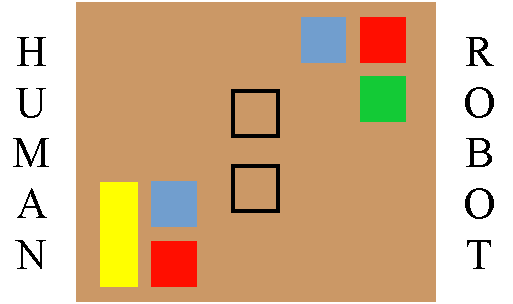
\includegraphics[scale=0.18]{figures/chapter2/task_setup_mini.pdf}}   
	\fancyhead[RO]{
\includegraphics[scale=0.20]{figures/chapter2/task_goal.pdf}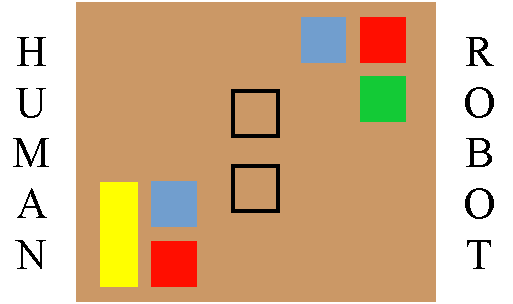
\includegraphics[scale=0.18]{figures/chapter2/task_setup_mini.pdf}\bfseries\thepage}  
	\fancyhead[RE]{\bfseries\nouppercase{\leftmark}}      % Chapter in the right on even pages
	\fancyhead[LO]{\bfseries\nouppercase{\rightmark}}     % Section in the left on odd pages
}%

\usepackage{pdfpages}
\usepackage{makecell}
\usepackage{pdflscape} 
\usepackage{mathtools}
\usepackage[section]{placeins}
\usepackage{afterpage}

%%%%%%%% my commands
\newcommand{\etal}{\textit{et al}.}
\newcommand{\ie}{\textit{i.e.}, }
\newcommand{\eg}{\textit{e.g.}, }
\newcommand{\fact}[3]{\mbox{\textit{#1}(#2, #3)}}
\newcommand{\circledtext}[1]{\raisebox{.5pt}{\textcircled{\raisebox{-.9pt} {#1}}}}
\newcommand{\sparql}{\textsc{SPARQL}}

\newcommand{\algConst}[1]{${\scriptscriptstyle #1}$}
\newcommand{\algNormTextSub}[2]{$\text{#1}_{#2}$}

\newcommand{\aslnumber}[1]{$#1$}
\newcommand{\aslstring}[1]{\textsf{#1}}
\newcommand{\aslvar}[1]{\textcolor{purple}{\textit{#1}}}
\newcommand{\asllabel}[1]{\textbf{#1}}
\newcommand{\annotation}[1]{{\footnotesize #1}}
\newcommand{\rulebody}[1]{\mbox{\hspace{.05\linewidth}}\begin{minipage}[t]{0.9\linewidth}#1.\end{minipage}}
\newcommand{\context}[1]{\begin{minipage}[t]{0.9\linewidth}#1\end{minipage}}
\newcommand{\planbody}[1]{\begin{minipage}[t]{0.9\linewidth}#1.\end{minipage}}
\newcommand{\Jason}[0]{\textbf{\textit{Jason}}}
\newcommand{\sn}{\mbox{\large\textbf{\texttt{\textasciitilde}}}}


\sloppy
\begin{document}
	\setcounter{chapter}{3} %% Numéro du chapitre précédent ;)
	\dominitoc
	\faketableofcontents
	\fi
	
	
\chapter{The central and pivotal role of Supervision}\label{chapter:chap4}
\minitoc
The supervision component is the binder of a robotic architecture. In this chapter, after a review of the state of the art, we will propose a set of requirements for interaction management: the needs and wants of a supervision system to manage interaction. Then, we will have a look on tools to implement such a supervision system.

\section{State of the art}\label{chap4:subsec:state_art_sup}
Without it, there is no task, no interaction happening, it controls the other components of the architecture. Indeed, what we define by `supervision', in the context of \acrshort{hri}, is the higher level of the architecture, the process involving real-time decision-making, eventually based on plans, and action execution and monitoring. When speaking about joint action, we think it is the component that should handle coordination, communication, monitoring, repair strategies and eventually joint attention and common ground alignment, based on shared representations.

We can find in the literature multiple work proposing components with a part of these features. The ones that we will present have been a source of inspiration, from far or close, for the contributions of this thesis. We will start with the oldest one, Shary, which has been developed in our laboratory. It is a component dedicated to supervision for human-robot interactions, with a strong emphasis on communication, allowing to execute shared plans and to monitor human and robot actions~\citep{clodic_2009_shary}. Chaski is a task-level executor, focusing on coordination and decision-making. It takes as input shared plans with deadlines and minimize the human idle time when executing of these plans~\citep{shah_2011_improved}. There is also Pike an online executive that unifies intention recognition and plan adaptation to deal with temporal uncertainties during Shared Plan execution~\citep{karpas_2015_robust}. \cite{gorur_2017_toward, gorur_2018_social} developed a robot able to handle unexpected human behavior, the first one being the human doing an action irrelevant to the task and the second one being the human not wanted the robot assistance. For this, they developed a human model and have a monitoring of human's actions and endow the robot with the abilities to be reactive and proactive. Similarly, \cite{baraglia_2017_efficient} proposed a reactive and proactive robot, being able to help when requested by the human or when detected. \cite{iocchi_2016_practical} presented a framework which generates and executes robust plans for service robots. It allows to not explicitly represent all possible situations the robot would face (\eg low battery means the robot should not navigate) and also to face unpredicted situations where an action failed with no alternative solutions. They implemented it by separating the state variables needed at both planning and execution and the one needed at execution time only. Finally, \cite{devin_2016_implemented} implemented a supervisor allowing the robot to estimate the human's mental state about the environment and the states of the goals, plans and actions, while executing shared plans.

\bigskip

It was difficult to find other works on decision-making and control dedicated to human-robot collaboration than the ones presented here, which shows that this subject is not tackled enough. First, it is not so often that complete robotic architectures run autonomously on a real robot and interact with a human. And, when they do, the supervision system is frequently not existing, the task being scripted, or is strongly designed for a specific task, preventing to be re-used in another context. Moreover, even when the work meets the criteria not scripted and not strongly built for a specific task such as the one of Iocchi \etal{}, there is no code or documentation to re-implement their system.


\section{The Needs and Wants of a supervision system to manage interaction} % Requirements

%\section{Design Methodology}

A part of the control features presented here is inspired by \cite{devin_2017_decisional}. Indeed, we intended to pursue her work, re-implementing a part of her software using Jason, a \acrshort{bdi} framework presented in Section~\ref{chap4:sec:bdi}, instead of if/else statements in C++, giving our software more flexibility, readability and genericity.
Then, to go further, we developed the \acrfull{jahrvis}\footnote{Also almost the acronym for ``Just A Rather Very Intelligent System'', see \url{https://en.wikipedia.org/wiki/J.A.R.V.I.S.}}, a more complete approach of a supervision component dedicated to \acrshort{hri} which tries to satisfy multiple requirements, trying to consider joint action as a whole:

\begin{bulletList}
	\item \textbf{Be generic}. The objectives developed in the rest of this list are valid for most collaborative tasks. Thus, it seemed essential for us to develop a software not dedicated to a particular human-robot task but able to handle plans for various tasks. 
	\item \textbf{Take into account the human partner}. In \acrshort{hri}, the human and the robot are partners. As seen in Section~\ref{chap1:sec:ja}, partners perform better when taking each other into account. Thus, by considering human abilities, perspective and mental states, the supervisor makes the robot a better partner for the human.
	\item \textbf{Leave decisions to the human}. In some cases, it is not useful, even counterproductive that the robot plans everything beforehand. Indeed, such elements such as the human action parameters, or who should execute a given action when it does not matter, or the order in which some actions should be executed, can be decided at execution time. Thus, we propose a supervisor handling two types of plan allowing to give latitude to human decisions and actions: conditional plans, and plans extending ``Agent X'' shared plans~\citep{devin_2017_decisions}.
	\item \textbf{Recognize human actions}. To monitor the plan progress, the robot should be able to monitor the human by recognizing their actions or being able to tell if they are idle.
	\item \textbf{Handle contingencies}. The robot has a shared plan, this is one thing, but to execute it and lead to the goal success is another one. Indeed, first, it is not sure that the human has exactly the same, and failures can happen. Therefore, sometimes not everything is like the robot had planned and the decision and execution manager has to tackle this. Thus, it should be able to handle a certain number of contingencies.
	\item \textbf{Manage relevant communications}. As stated in Section~\ref{chap1:sec:comm}, communication is one of the keys of collaboration. Therefore, it is important to endow the robot with the ability to manage relevant communication actions, verbal and non-verbal.
	\item \textbf{Consider the interaction outside collaborative tasks} A robot dedicated to collaborative tasks, in a real-life context, will interact with humans outside or between these tasks. We propose to consider this fact by defining what we called \textit{interaction sessions}. An interaction session gives a frame to the interaction and allows to take into account a number of facts from one task to another or from one session to another.
	\item \textbf{Adapt to the human experience, abilities or preferences}. Humans are all different, because of their experience, abilities or preferences among other things. A robot taking into account its previous interactions with a human (\eg behaving differently with a novel user or an experienced user) or adapting to their abilities (\eg some people cannot climb stairs, a robot guide can indicate the elevator instead) will improve the efficiency and the quality of the interaction, and the user's experience.
\end{bulletList}


\section{Which tool to implement a supervision?}\label{chap4:sec:bdi}

In this section, we will present the framework we chose as a base for our supervision software. First, we explain how we did this choice and then the internal mechanisms of the framework. The supervision component itself, \acrshort{jahrvis}, we will be presented in the next Chapters.

\subsection{The Choice of the Programming Framework}

% mettre un petit paragraphe pour citer 
% citer RAE (papier Survey de Malik et Felix sur les HTN pour la robotique) et PRS, CRAM (pas de mécanismes de décision en ligne, ni de reprise d'erreur), JASON? + aucun de ces systèmes ne font de l'interaction humain robot
% difficulté de la planification d'un côté et de l'exécution du plan de l'autre
% l'originalité de JAHRVIS c'est de faire une exécution pour l'humain et le robot (avec les beliefs etc)

Restart from scratch or base oneself work on an existing software? This is the question which has been studied at the beginning of this thesis work about the implementation of the supervision software. It was possible 
\begin{inlineEnumerate}
	\item to develop the wanted features using the code\footnote{\url{https://github.com/laas/supervisor}} of the previous PhD student working on the supervision, Sandra Devin,\label{chap4:list:sandra}
	\item to choose among existing software dedicated to decision and execution for Human-Robot Interaction,\label{chap4:list:soft_hri}
	\item to choose among existing software dedicated to decision and execution for robotic platforms, and\label{chap4:list:robot}
	\item to develop a new software from scratch.\label{chap4:list:new}
\end{inlineEnumerate}

The obvious drawback of \ref{chap4:list:new} is that it takes a lot of time to start a new software from scratch and that it often leads to reinvent the wheel. Then, first we looked at existing solutions. Concerning the possibility \ref{chap4:list:sandra}, Devin had developed interesting features, but the code is not modular and it was difficult to add new features or to modify the existing ones without breaking everything. Thus, there was the solutions \ref{chap4:list:soft_hri} and \ref{chap4:list:robot} left. When looking for existing software to manage human-robot interactions, we could not find any open-source one with a minimum of features, documentation and not entirely dedicated to a given task. Therefore, we turned ourselves toward robotic framework. We compared existing open-source decision-making and execution software for robots. To cite a few, there is the PetriNetPlans library introduced by \cite{ziparo_2011_petri} which is a framework for planning and execution. \cite{beetz_2010_cram} developed CRAM, a software implementing reasoning mechanisms that can infer control decisions. A framework to implement hierarchical state machines is available among ROS libraries, SMACH\footnote{\url{http://wiki.ros.org/smach}}, defined as ``task-level architecture for rapidly creating complex robot behavior''. Or, a C++ library to create behavior trees has been developed, called BehaviorTree.CPP~\footnote{\url{https://github.com/BehaviorTree/BehaviorTree.CPP/}}. Finally, there are several implementations of the \acrshort{bdi} model presented in Section~\ref{chap3:sec:archi} such as JAM~\citep{huber_1999_jam}, Jadex~\citep{braudach_2005_jadex}, SPARK~\citep{morley_2004_spark}, dMARS~\citep{dinverno_1998_formal}, OpenPRS~\citep{ingrand_1996_prs} or Jason~\citep{bordini_2007_jason}. 

As a first step, for prototyping and respecting project deadlines, our choice went to SMACH because its compatibility with ROS and its facility to be used. Then, it was no surprise, it became more and more difficult to program complex robot behaviors, state machines were not enough powerful. Thus, we examined possibilities for our second choice. After a comparison considering potential compatibility with ROS, possible integration with the other software of our architecture, availability of documentation, users' feedbacks, maintenance, and possibility of code modifications, our choice went to Jason designed by \cite{bordini_2007_jason} which is a Java interpreter of AgentSpeak created by \cite{rao_1996_agentspeak}. It has the advantage to be a \acrshort{bdi} (Beliefs, Desires, Intentions, see Section~\ref{chap3:sec:archi}) agent-oriented framework, fitting with our architecture. The \acrshort{bdi} framework implements a process, called the reasoning cycle or more commonly the sense-decide-act cycle~\citep{albus_1991_outline}, deciding step by step, which action to perform to reach a goal. It allows more modularity than state machines to handle contingencies and events. It also facilitates reasoning on agents' -- humans and robot -- beliefs. We chose this framework among the \acrshort{bdi} ones and not another because it is implemented in Java and thus was compatible with rosjava\footnote{\url{https://github.com/rosjava/rosjava_core}} (\ie ROS implementation in Java), it is still developed and maintained, it is well documented (theoretically~\citep{bordini_2007_jason} and implement-ally\footnote{\url{http://jason.sourceforge.net/api/}}) which allows source code understanding and modifications, and there is a mailing list for users and its archives available\footnote{\url{https://sourceforge.net/p/jason/mailman/jason-users/}}.

\subsection{Programming with Jason}\label{chap4:subsec:jason}
As said above, Jason is a \acrshort{bdi}-based framework, allowing what is called \textit{agent-oriented programming}. Originally designed for multi-robot programming, it can be used for other purposes such as ours. How does it work?

We explained in Section~\ref{chap3:sec:archi} that there were three main concepts involved in \acrshort{bdi} models: beliefs, desires and intentions. Well, Jason's purpose is to program agents. Thus, each agent has beliefs, desires and intentions. The beliefs are what it perceives, acquires from other agents and computes. They can produce desires, \ie states of affairs the agent wants to achieve. Then, the agent deliberates on its desires and choose to commit to some of them, \ie the chosen desires become intentions. To satisfy its intentions, the agent executes procedural programs, called plans, leading to actions. The procedural knowledge is written by the programmer.

The programming of the behavior of an agent is in the AgentSpeakLanguage (ASL). The program is designed by a user, a programmer. A program contains, among other things, plans. These plans have actions. An action is described by a Java program, written by the Jason's user. Then, to run, a program uses the decision loop, so called the \textit{reasoning cycle}, integrated to Jason. It is possible to customize some functions of the reasoning cycle by overloading or adding Java functions of the agent's constructors, belief base and reasoning cycle. 

\subsubsection{Agents} In the ASL program of an agent, it is possible to see plans, beliefs, desire and test goal. First, let's see a very simple example of program with the agent Bob\footnote{\url{http://jason.sourceforge.net/mini-tutorial/hello-bdi/}}, presented in Listing~\ref{chap4:lst:bob}. Bob has one initial (\ie given by the programmer, not acquired by perception) belief which is |happy(bob)|. A belief is a property, here |happy|, which can have whatever number of arguments (including zero), here |bob| and a source (\eg |source(percept)| means that the belief has been acquired through perception, |source(self)| means that it has been computed by the agent itself and |source(alice)| means that it has been received from the agent Alice). Then, he has one initial desire which is recognizable by |!|. And finally, he has a plan allowing to achieve the desire |say(hello)|. A plan is triggered by an event, here |+!say(X)| (\ie the event is that the goal |say(hello)| has been added), has a context (\ie a precondition), here |happy(bob)| and has a body which contains the actions to execute, here |.print(X)| (with |X| being a variable -- variables have their first letter in upper case). If we remove the initial belief |happy(bob)| from the first line, as the program is written and considering that Bob is the only agent, he cannot print hello, as the precondition of the plan will not be true.

\begin{lstlisting}[caption={ASL program of Bob, a Jason agent}, label={chap4:lst:bob}]
happy(bob).	\\belief

!say(hello).	\\desire

\\plan
+!say(X) : happy(bob) <- 
	.print(X).		
\end{lstlisting} 

In another example, illustrated by Listing~\ref{chap4:lst:bobalice}, Bob has no initial belief nor initial goal. He has plans for two events: starting to believe he is happy and having the goal to say hello. We can see that there is also a program for another agent, Alice. She has an initial goal, her, which is to inform bob that he is happy. Therefore, we can see that an agent can add a belief in another agent's belief base. When Bob gets the information that he is happy, this triggers his first plan, creating for him the goal |!say(hello)|. As Bob does not believe that today is Monday, he can trigger his second plan to say hello. In this plan, there are three elements: a print action, a wait action and the addition of a new goal. And thus, here, we are in the presence of a recursive plan which never ends. 

\begin{lstlisting}[caption={ASL programs of Bob and Alice, two Jason agents}, label={chap4:lst:bobalice}]
\\bob.asl
\\for example purposes, the precondition is true
\\but it can be logical expressions with beliefs,
\\functions...
+happy(bob) : true <- 
	!say(hello).

+!say(X) : not today(monday) <- 
	.print(X); 
	.wait(500); 
	!say(X).

\\alice.asl
!inform.

+!inform : true <- .send(bob,tell,happy(bob)).
\end{lstlisting} 

\subsubsection{Actions} To give an idea of what looks like the Java program of an action, here is an example of a Java function for the action |.print| in Listing~\ref{chap4:lst:print}.

\begin{lstlisting}[caption={.print action}, label={chap4:lst:print}, language=Java]
public class print extends DefaultInternalAction {
	@Override
	public Object execute(TransitionSystem ts, Unifier un, Term[] args) throws Exception {
		String sout = argsToString(args);
		System.out.print(sout.toString() + "\n");
	}
	return true;
	}
}
\end{lstlisting} 

In Jason, there are two types of actions defined: \emph{environment actions} and \emph{internal actions}. \emph{Environment actions} allow an agent to act within its environment, usually producing effects visible by other agents. Whereas, \emph{internal actions} are designed to be run internally within an agent such as the print action and can be used to return values or booleans. When being executed, there are not handled the same way in the Jason's reasoning cycle. The definition of which type an action should be falls to the programmer, which should choose according to their need.

We have seen what looks like the program of Jason agent. Now, we are going to see how it is run by the Jason interpreter.


\subsubsection{Reasoning cycle} Each agent has what has been coined a \textit{reasoning cycle}, composed of 10 steps. It resembles a decision loop, running each step one by one and starting again at the first one. The steps 1 to 4 are dedicated to the belief update of the agent. The steps 5 to 10 describe the interpretation of the ASL program. In these latter, an event is selected, as well as a plan corresponding to this event and then the first formula (\eg an action or a goal) of the plan is executed. It is illustrated by Figure~\ref{chap4:fig:jason_cycle}. The steps are the following ones, in this order:
\begin{enumerate}
	\item Perceiving the Environment: Each agent has a Java function called |perceive|. This function can retrieve data from a simulated environment or be customized by the programmer to get actual perception data. The function outputs a list of beliefs, along with their source (\eg |<isOn(box1,table)[source(percept)]|, |color(box1,red)[source(percept)]>|).
	\item Updating the Belief Base: The agent's belief base is updated with the perception data. Each change in the belief base generates an event (\eg |+color(box1,red)[source(percept)]| and if later the color of the box is not part of the perception data anymore, it will be |-color(box1,red)[source(percept)]|).\label{chap4:list:update_bb}
	\item Receiving Communication from Other Agents: It checks if an agent received a message from another agent such as the message Bob received from Alice in Listing~\ref{chap4:lst:bobalice}. A message can be a belief, a plan, a goal or a questioning on a given belief.
	\item Selecting ‘Socially Acceptable’ Messages: It is a function the programmer should customize. It allows agent to refuse messages or types of message from some given agents based on some rules written in Java by the programmer, \eg no message from the agent Alice.
	\item Selecting an Event: Events are either perceived changes in the environment or changes in the agent's own goals. There is a queue of events and at each reasoning cycle only one is selected to be handled. The default method to select it is a FIFO but, as every function of the reasoning cycle, it can be customized. 
	\item Retrieving all Relevant Plans: From the selected event, it tries to find all the relevant plans for this event, in the plan library, \ie the plans written by the programmer in ASL. The function tries to find the plans that can be \textit{unified} with event, \ie the ones with their left part (the trigger) matching the event. For example, if the selected event is |+color(box1,red)[source(percept)]| and in the plan library there are these six plans:
\begin{lstlisting}[style=inline]
+position(Object,Coords) : true <- .print(Coords).
+color(Object,red) : true <- .print(nice).
+color(Object,red)[source(self)] : true <- .print(nice).
+color(box1,Color) : true <- .print(nice).
+color(Object,Color) : false <- .print(Color).
+color(Object,blue) : true <- .print(so-so).
\end{lstlisting}
	then there are three relevant plans (the last one is also relevant because what is looked for here is the triggers only and not the preconditions):
\begin{lstlisting}[style=inline]
+color(Object,red) : true <- .print(nice).
+color(box1,Color) : true <- .print(nice).
+color(Object,Colour) : false <- .print(Colour).
\end{lstlisting}
	\item Determining the Applicable Plans: It takes the list of relevant plans and sees which ones are applicable. To do so, it looks at the context (the preconditions) of the plans. The context can be beliefs, prolog-like rules, internal actions, logical expressions or booleans. If we look at the example of the previous step, there were three relevant plans. Their contexts are simple booleans. Two of them are true, the other one is false, thus the two first plans are applicable.
	\item Selecting One Applicable Plan: It takes the list of applicable plans and selects the one that will be elected to become an intention, \ie to be executed. As usual, this is a customizable function for which the default behavior is to take the first plan in the order of the plan library, \ie in the order written by the programmer. Still with the same example, thus, the one plan to be selected is the first one, |+color(Object,red) : true <- .print(nice).| If the event was external, \ie from perception, it creates a new intention, adding it to the set of intentions. Then, the agent has a new \textit{focus of attention}. If the event was internal, \eg a belief addition inside a plan, then the selected plan is added on the top of the existing intention. 
	\item Selecting an Intention for Further Execution: As seen in the previous step, an agent can have more than one intention in the set of intentions, each representing a different focus of attention. Then, at this step is chosen the intention of which the formula will be executed. The default function chooses the first intention of the list. After execution of the formula, the intention will go at the end of the intentions list.
	\item Executing One Step of an Intention: The first formula of the selected intention is executed (this number is also customizable and the programmer can choose that an agent execute more than once formula in the same reasoning cycle). It can be an internal action, an environment action, a goal, a belief addition or deletion and two other types that will not be developed here. 
\end{enumerate}

Therefore, each agent has a reasoning cycle running repeatedly, independent from the other agents' reasoning cycle. Interactions between each agent happen through the messages they send to each other's and eventually the effects they produce on the environment which are then perceived by the other agents. 


\begin{landscape}
\begin{figure}
	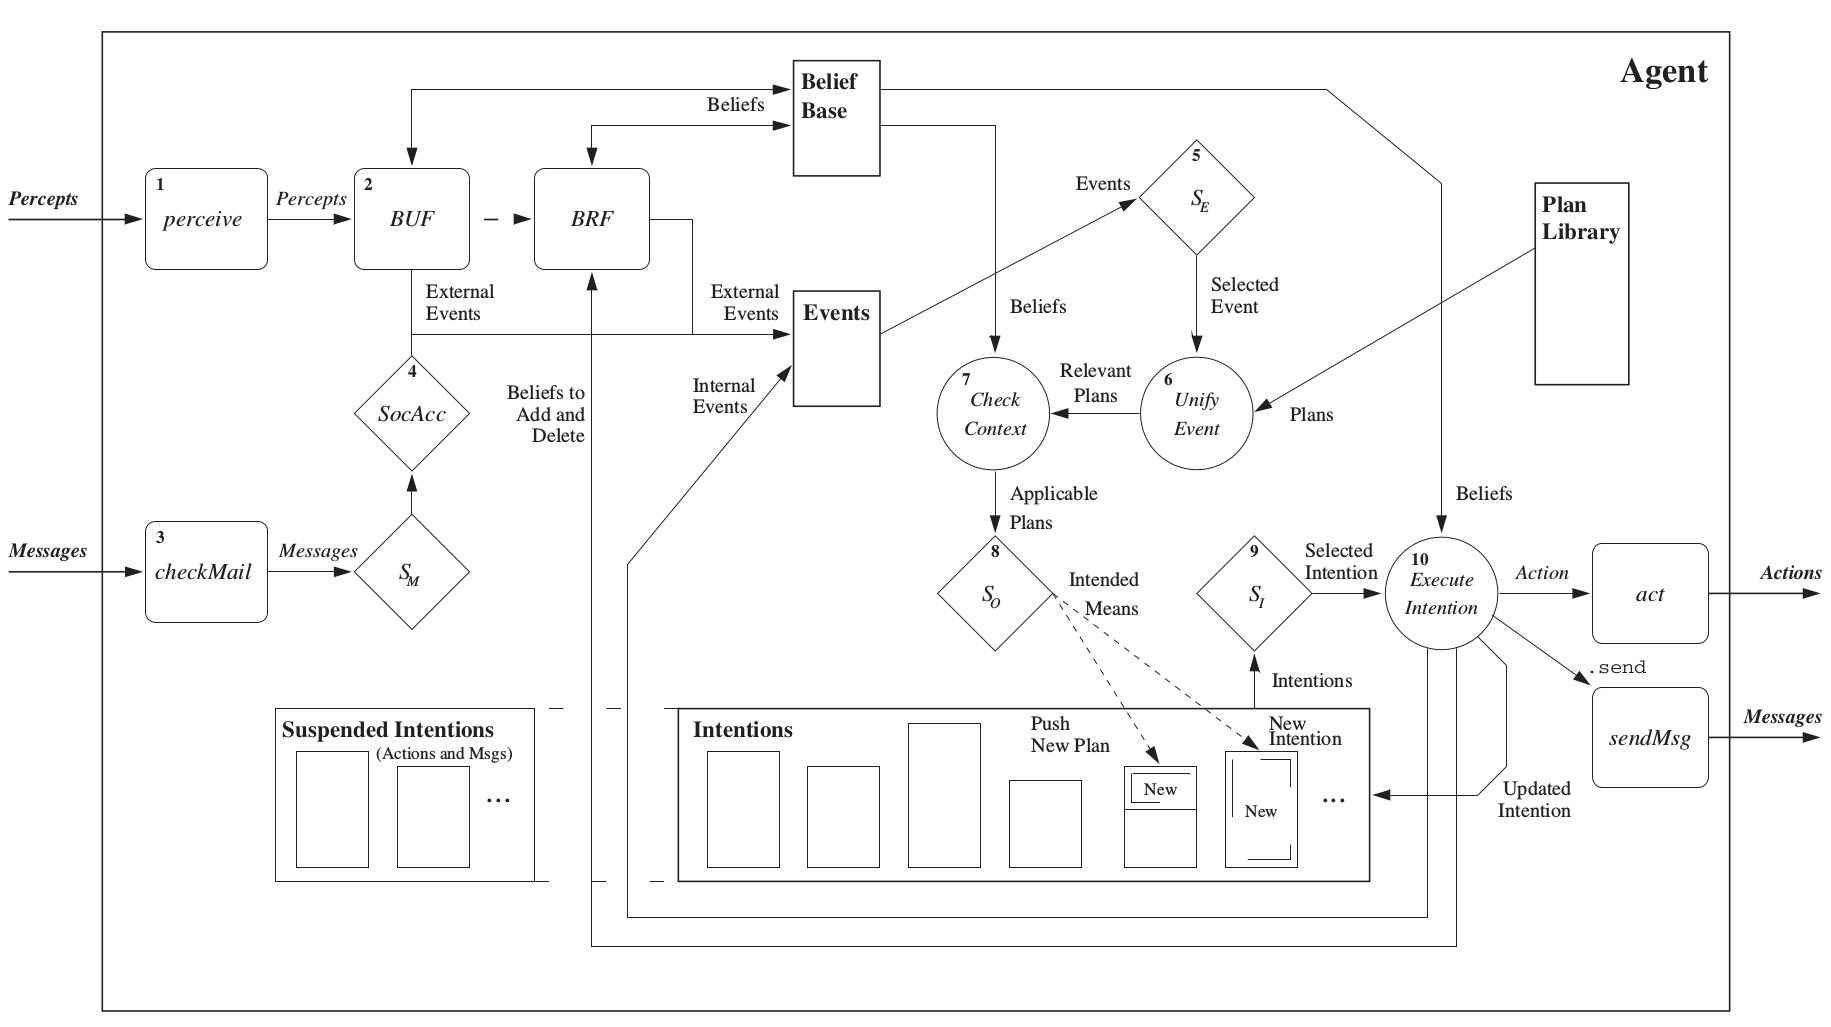
\includegraphics[width=\linewidth]{figures/chapter2/jason_cycle.png}
	\caption{The Jason reasoning cycle~\citep{bordini_2007_jason}. Each step presented above has its numbered corresponding box.}
	\label{chap4:fig:jason_cycle}
\end{figure}
\end{landscape}

\subsubsection{Plan failure handling}

For the case where a plan fails (\eg an action fails -- there are other reasons for which a plan could fail but we will not discuss the details here), Jason integrates a mechanism handling failures. It consists in cancel the execution of the plan and generating a triggering event for a contingency plan whose prefix is |-!|. If the contingency plan can be found -- written by the programmer --, it is executed. Then, if the plan which originally failed was a subplan of another plan, this plan will continue normally. 

An illustration is given in Listing~\ref{chap4:lst:failure}. The result of the execution of this agent file would be the printing ``unknown error'' and then ``bye'' in case of the failure of the |robot_speech| action execution with an instantiated speech module. Indeed, the initial goal |speak| creates the subgoal |say_hello|. Unfortunately, the action |robot_speech| fails with an empty error message, generating the event |-!say_hello[error_msg(Msg)]|. There are two plans for this event but as |Msg=""|, the second one is chosen, printing ``unknown error''. Then, |speak| continues in the same way it does when goal |say_hello| is achieved successfully, printing ``bye''.

\begin{lstlisting}[caption={Example of plan failure handling}, label={chap4:lst:failure}]
!speak.

+!speak : true <- 
	!say_hello;
	.print(bye).

+!say_hello : true <-
	robot_speech(hello);
	.print(hello).

-!say_hello[error_msg(Msg)] : .substring(Msg,no_speech_found) <-
	.print(no speech module was found).

-!say_hello[error_msg(Msg)] : true <-
	.print(unknown error).	
\end{lstlisting} 

\subsection{Jason Integration with ROS}
The robotic architecture presented in Section~\ref{chap3:sec:rob_archi} uses the ROS framework~\citep{quigley_2009_ros} to enable communication between its components. Thus, to be able to build a supervision software based on Jason, we needed to interface it with ROS as well. At the time, there was no available bridge between Jason and ROS, Jason being extensively used in simulation contexts. Thus, we developed our own -- and at about the same moment, the Jason's developers started to develop theirs~\citep{silva_2020_embedded} (what we realized a bit later), both using rosjava. We tackled the problem in very different ways. A user of their implementation only needs to fill one perception (topics) and one action (topics/services) manifests to link the system with ROS and then implement their agent in ASL. Thus, it is quite easy to use. However, it has drawbacks. Therefore, action requests are directly sent from ASL to the hardware controller, with no possibility of Java processing. Moreover, action status/result can only be boolean which is not enough for a system like ours needing to perform service queries of data to the external Knowledge Base for example. Finally, there is no bridge with action servers which are often used for motion planers for example. 

\begin{figure}[!ht]
	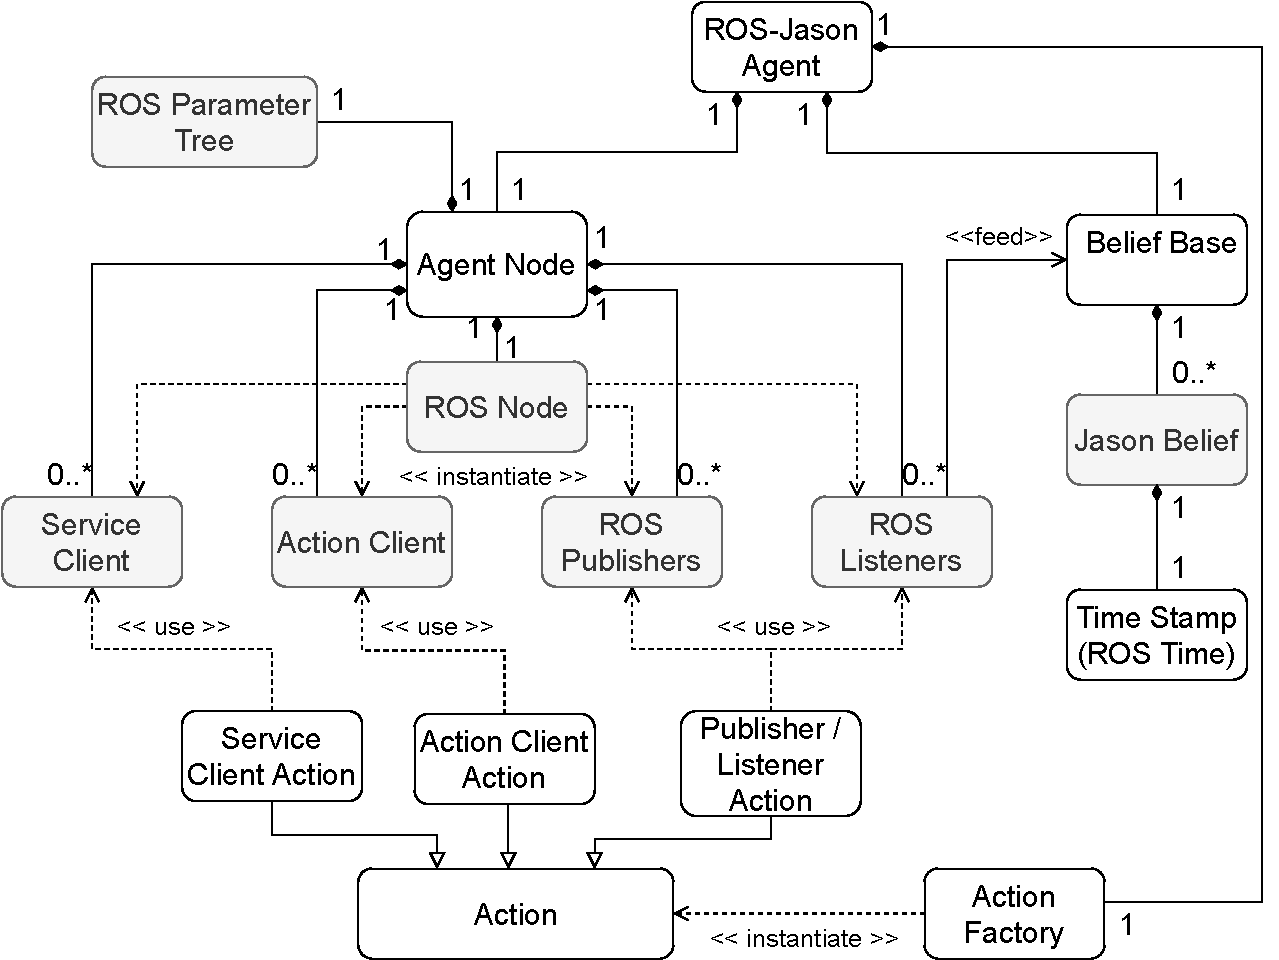
\includegraphics[width=\linewidth]{figures/chapter2/RJS_diagram.pdf}
	\caption{Simplified Java class diagram of our ROS-Jason implementation. In white are our customized classes and in grey the native ROS and Jason classes.}
	\label{chap4:fig:rjs}
\end{figure}

A simplified Java class diagram of our  implementation\footnote{\url{https://github.com/amdia/rjs}} is presented in Figure~\ref{chap4:fig:rjs}. We defined for each Jason agent a customized Java class (\acrfull{rja} on the figure) which has an Agent Node, an action factory and a belief base where all beliefs are time stamped with the roscore time. 

An Agent Node has an attribute, the ROS Parameter Tree, allowing to load YAML parameters from files in which, among other things, are written services, topics and action servers info, as shown in Listing~\ref{chap4:lst:ros-jason}, a bit similarly to the manifests of~\cite{silva_2020_embedded}. From these parameters, the Agent Node can automatically instantiate all the needed ROS components through its ROS node. 

\begin{lstlisting}[caption={Example of service, topic and action server definitions in a YAML file.}, label={chap4:lst:ros-jason}]
services:
	onto_individual: 
		name: /ontologenius/individual/robot
		type: ontologenius/OntologeniusService
	onto_class: 
		name: /ontologenius/class/robot
		type: ontologenius/OntologeniusService
topics:
	mementar_occasions: 
		name: /mementar/occasions/robot
		type: mementar/MementarOccasion
		function: sub
	plan_request:
		name: /planner/request_new_plan
		type: planner_msgs/PlanRequest
		function: pub
action_servers:
	plan_motion: /pr2_tasks_node/plan
	execute_motion: /pr2_tasks_node/execute
\end{lstlisting}


An \acrshort{rja} can receive perception updates (from other components of the robotic architecture) in its Belief Base through ROS topic listeners. Moreover, we customized\footnote{This modification of the belief update function is not part of our ROS-Jason implementation but is on top of it, in the \acrshort{jahrvis} implementation which relies on ROS-Jason.} the belief update function (step~\ref{chap4:list:update_bb} of the reasoning cycle) as we chose to abandon a state-based perception to adopt an event-based perception. So, percepts are not elements that when perceived at time T are added to the belief base and disappearing when not perceived anymore at time T+1. There are now updates (additions and deletions) from the external Knowledge Base, in this way, it limits the number of message exchanges, \ie instead of receiving every 500 ms for 10 seconds that the agent perceives |cube_1|, it receives for example an addition at t=18s and a deletion at t=28s. 

To each belief added in the belief base, from perception or internal computation, is added a time stamp from the current ROS time. Currently, it is useful for the computation of the Quality of Interaction presented in Chapter~\ref{chapter:chap7} and also to feed the \acrshort{kb} timeline and for debugging.

An \acrshort{rja} has an Action Factory -- abstract in the ROS-Jason framework and instantiated in \acrshort{jahrvis} -- containing the list of environment actions it can perform -- in the case of our architecture, not all actions of this type are for the robot to act on its environment, sometimes there are queries to other components of the architecture. The Action Factory instantiates the Action called through the ASL program at execution time. An Action can either be based on a ROS service client, or an ROS action client, or a ROS publisher for the request and a ROS listener for the result. 

\section{Conclusion}

In this chapter, we laid the foundations for our supervision component, \acrshort{jahrvis}. First, we presented what we expected of such a component dedicated to human-robot collaboration: to be generic, to take into account the human partner, to leave decisions to them, to monitor human actions, to handle contingencies, to manage relevant communications, to consider the interaction outside collaborative tasks, and to adapt to the human experience, abilities or preferences.

Then, we presented Jason, the programming framework on which we chose to base on \acrshort{jahrvis}. Relying on the \acrshort{bdi} model, it allows to implement complex reasonings what is suitable for our needs. A Jason agent has a library of plans written in ASL, a belief base and a set of intentions containing the next step of plans it should perform. It has a reasoning cycle, continuously receiving updates from the world state from the robotic architecture \acrshort{kb}s and re-evaluating which Jason action or plan should be executed. In Chapter~\ref{chapter:chap6}, we will see that each feature of \acrshort{jahrvis} is implemented with a Jason agent, or more precisely with a \acrfull{rja}. Indeed, ROS is the chosen middleware to enable communication between the components of the robotic architecture. Thus, we needed to build a bridge between ROS and Jason. 


\ifdefined\included
\else
\bibliographystyle{acm}
\bibliography{These}
\end{document}
\fi